% !TeX spellcheck = es_ES
% !TeX encoding = UTF-8
\documentclass[10pt, a4paper, landscape]{article}

% ----- packages -----
\usepackage{amsmath} % AMS mathematical facilities for LaTeX
\usepackage{amssymb}
\usepackage{enumitem} % Control layout of itemize, enumerate, description
\usepackage{fancyhdr} % Extensive control of page headers and footers in LaTeX2
\usepackage{geometry} % Flexible and complete interface to document dimensions
\usepackage{graphicx} % Enhanced support for graphics
\usepackage{hyperref} % Extensive support for hypertext in LaTeX
\usepackage{multicol} % Intermix single and multiple columns
\usepackage{parskip} % Layout with zero \parindent, non-zero \parskip
\usepackage{tikz} % Create PostScript and PDF graphics in TeX
\usepackage{titlesec} % Select alternative section titles

% ----- pdf metadata -----
\hypersetup{
	pdftitle={Hoja de Referencia Adicional},
	pdfsubject={The Econometrics Cheat Sheet Project - marcelomijas - CC-BY-4.0},
	pdfauthor={Marcelo Moreno Porras},
	pdfkeywords={statistics, latex, economics, cheatsheet, econometrcis, ols-regression, economic-modelling},
	pdfduplex={DuplexFlipShortEdge}
}

% ----- random seed -----
\pgfmathsetseed{10}

% ----- custom commands -----
\DeclareMathOperator{\E}{E}
\DeclareMathOperator{\Var}{Var}
\DeclareMathOperator{\se}{ee}
\DeclareMathOperator{\Cov}{Cov}
\DeclareMathOperator{\Corr}{Corr}
\DeclareMathOperator{\rk}{rg}
\DeclareMathOperator{\Cr}{Cr}
\DeclareMathOperator{\AIC}{AIC}
\DeclareMathOperator{\HQ}{HQ}
\DeclareMathOperator{\BIC}{BIC}
\newcommand{\SSR}{\text{SRC}}
\newcommand{\SSE}{\text{SEC}}
\newcommand{\SST}{\text{STC}}
\newcommand{\trend}{\text{Tend}_{t}}
\newcommand{\const}{\text{const}}

% ----- page customization -----
\geometry{margin=1cm} % margins config
\pagenumbering{gobble} % remove page numeration
\setlength{\parskip}{0cm} % paragraph spacing
% title spacing
\titlespacing{\section}{0pt}{2ex}{1ex}
\titlespacing{\subsection}{0pt}{1ex}{0ex}
\titlespacing{\subsubsection}{0pt}{0.5ex}{0ex}

% ----- footer -----
\pagestyle{fancy}
\renewcommand{\headrulewidth}{0pt}
\cfoot{\href{https://github.com/marcelomijas/econometrics-cheatsheet}{\normalfont \footnotesize ADD-25.08.1-ES - github.com/marcelomijas/econometrics-cheatsheet - Licencia CC-BY-4.0}}
\setlength{\footskip}{12pt}

% ----- document -----
\begin{document}

\begin{multicols}{3}

\begin{center}
	\textbf{\LARGE \href{https://github.com/marcelomijas/econometrics-cheatsheet}{Hoja de Referencia Adicional}}

	{\footnotesize Por Marcelo Moreno Porras - Universidad Rey Juan Carlos}

	{\footnotesize The Econometrics Cheat Sheet Project}
\end{center}

\section*{Notación matricial MCO}

El modelo econométrico general:

\begin{center}
	\( y_{i} = \beta_{0} + \beta_{1} x_{1i} + \cdots + \beta_{k} x_{ki} + u_{i} \)
\end{center}

Puede ser escrito en notación matricial como:

\begin{center}
	\( y = X \beta + u \)
\end{center}

Llamemos \( \hat{u} \) al vector de residuos estimados \( (\hat{u} \neq u) \):

\begin{center}
	\( \hat{u} = y - X \hat{\beta} \)
\end{center}

El \textbf{objetivo} de MCO es \textbf{minimizar} la \( \SSR \):

\begin{center}
	\( \min \SSR = \min \sum_{i = 1}^{n} \hat{u}_{i}^{2} = \min \hat{u}^{\top} \hat{u} \)
\end{center}

\begin{itemize}[leftmargin=*]
	\item Definiendo \( \hat{u}^{\top} \hat{u} \):
	\begin{center}
		\( \hat{u}^{\top} \hat{u} = (y - X \hat{\beta})^{\top} (y - X \hat{\beta}) \)

		\( = y^{\top} y - 2 \hat{\beta}^{\top} X^{\top} y + \hat{\beta}^{\top} X^{\top} X \hat{\beta} \)
	\end{center}
	\item Minimizando \( \hat{u}^{\top} \hat{u} \):
	\begin{center}
		\( \frac{\partial \hat{u}^{\top} \hat{u}}{\partial \hat{\beta}} = -2 X^{\top} y + 2 X^{\top} X \hat{\beta} = 0 \)

		\( \hat{\beta} = (X^{\top} X)^{-1} (X^{\top} y) \)

		\scalebox{0.85}{
			\(
			\begin{bmatrix}
				\beta_{0} \\
				\beta_{1} \\
				\vdots    \\
				\beta_{k}
			\end{bmatrix}
			=
			\begin{bmatrix}
				n          & \sum x_{1}       & \hdots & \sum x_{k}       \\
				\sum x_{1} & \sum x_{1}^{2}   & \hdots & \sum x_{1} x_{k} \\
				\vdots     & \vdots           & \ddots & \vdots           \\
				\sum x_{k} & \sum x_{k} x_{1} & \hdots & \sum x_{k}^{2}
			\end{bmatrix}^{-1}\cdot
			\begin{bmatrix}
				\sum y       \\
				\sum y x_{1} \\
				\vdots       \\
				\sum y x_{k}
			\end{bmatrix}
			\)
		}
	\end{center}
	La segunda derivada \( \frac{\partial^{2} \hat{u}^{\top} \hat{u}}{\partial \hat{\beta}^{2}} = X^{\top} X > 0 \) (es un mín.)
\end{itemize}

\section*{Matriz de varianzas-covarianzas de \( \hat{\beta} \)}

Tiene la siguiente forma:

\begin{center}
	\( \Var(\hat{\beta}) = \hat{\sigma}_{u}^{2} \cdot (X^{\top} X)^{-1} \)
\end{center}

\begin{center}
	\scalebox{0.85}{ 
		\( =
		\begin{bmatrix}
			\Var(\hat{\beta}_{0})                  & \Cov(\hat{\beta}_{0}, \hat{\beta}_{1}) & \hdots & \Cov(\hat{\beta}_{0}, \hat{\beta}_{k}) \\
			\Cov(\hat{\beta}_{1}, \hat{\beta}_{0}) & \Var(\hat{\beta}_{1})                  & \hdots & \Cov(\hat{\beta}_{1}, \hat{\beta}_{k}) \\
			\vdots                                 & \vdots                                 & \ddots & \vdots                                 \\
			\Cov(\hat{\beta}_{k}, \hat{\beta}_{0}) & \Cov(\hat{\beta}_{k}, \hat{\beta}_{1}) & \hdots & \Var(\hat{\beta}_{k})
		\end{bmatrix}
		\)
	}
\end{center}

\quad donde: \( \hat{\sigma}_{u}^{2} = \frac{\hat{u}^{\top} \hat{u}}{n - k - 1} \)

Los errores estándar están en la diagonal de:

\begin{center}
	\( \se(\hat{\beta}) = \sqrt{\Var(\hat{\beta})} \)
\end{center}

\section*{Medidas de error}

\begin{itemize}[leftmargin=*]
	\item \( \SSR = \hat{u}^{\top} \hat{u}= y^{\top} y - \hat{\beta}^{\top} X^{\top} y = \sum(y_{i} - \hat{y}_{i})^{2} \)
	\item \( \SSE = \hat{\beta}^{\top} X^{\top} y - n \overline{y}^{2} = \sum(\hat{y}_{i} - \overline{y})^{2} \)
	\item \( \SST = \SSR + \SSE = y^{\top} y - n \overline{y}^{2} = \sum(y_{i} - \overline{y})^{2} \)
\end{itemize}

\columnbreak

\section*{Matriz de varianzas-covarianzas de \( u \)}

Tiene la siguiente forma:

\begin{center}
	\( \Var(u) = \)
	\scalebox{0.85}{
		\(
		\begin{bmatrix}
			\Var(u_{1})        & \Cov(u_{1}, u_{2}) & \hdots & \Cov(u_{1}, u_{n}) \\
			\Cov(u_{2}, u_{1}) & \Var(u_{2})        & \hdots & \Cov(u_{2}, u_{n}) \\
			\vdots             & \vdots             & \ddots & \vdots             \\
			\Cov(u_{n}, u_{1}) & \Cov(u_{n}, u_{2}) & \hdots & \Var(u_{n})
		\end{bmatrix}
		\)
	}
\end{center}

Bajo no heterocedasticidad y no autocorrelación, la matriz de varianzas-covarianzas:

\begin{center}
	\( \Var(u) = \sigma_{u}^{2} \cdot I_{n} = \)
	\scalebox{0.85}{
		\(
		\begin{bmatrix}
			\sigma_{u}^{2} & 0              & \hdots & 0              \\
			0              & \sigma_{u}^{2} & \hdots & 0              \\
			\vdots         & \vdots         & \ddots & \vdots         \\
			0              & 0              & \hdots & \sigma_{u}^{2}
		\end{bmatrix}
		\)
	}
\end{center}

\quad donde \( I_{n} \) es una matriz identidad con \( n \times n \) elementos.

Bajo \textcolor{cyan}{\textbf{heterocedasticidad}} y \textcolor{magenta}{\textbf{autocorrelación}}, la matriz de varianzas-covarianzas:

\begin{center}
	\( \Var(u) = \sigma_{u}^{2} \cdot \Omega = \)
	\scalebox{0.85}{
		\(
		\begin{bmatrix}
			\textcolor{cyan}{\sigma_{u_{1}}^2}   & \textcolor{magenta}{\sigma_{u_{12}}} & \hdots & \textcolor{magenta}{\sigma_{u_{1n}}} \\
			\textcolor{magenta}{\sigma_{u_{21}}} & \textcolor{cyan}{\sigma_{u_{2}}^2}   & \hdots & \textcolor{magenta}{\sigma_{u_{2n}}} \\
			\vdots                               & \vdots                               & \ddots & \vdots                               \\
			\textcolor{magenta}{\sigma_{u_{n1}}} & \textcolor{magenta}{\sigma_{u_{n2}}} & \hdots & \textcolor{cyan}{\sigma_{u_{n}}^2}
		\end{bmatrix}
		\)
	}
\end{center}

\quad donde \( \Omega \neq I_{n} \).

\begin{itemize}[leftmargin=*]
	\item Heterocedasticidad: \( \Var(u) = \sigma_{u_{i}}^{2} \neq \sigma_{u}^{2} \)
	\item Autocorrelación: \( \Cov(u_{i}, u_{j}) = \sigma_{u_{ij}} \neq 0, \; \forall i \neq j \)
\end{itemize}

\section*{Omisión de variables}

Casi siempre es difícil disponer de todas las variables relevantes. Por ejemplo, un modelo con todas las variables:

\begin{center}
	\( y = \beta_{0} + \beta_{1} x_{1} + \beta_{2} x_{2} + v \)
\end{center}

\quad donde \( \beta_{2} \neq 0 \), \( v \) el término de error y \( \Cov(v \mid x_{1}, x_{2}) = 0 \).

El modelo con las variables disponibles:

\begin{center}
	\( y = \alpha_{0} + \alpha_{1} x_{1} + u \)
\end{center}

\quad donde \( u = v + \beta_{2} x_{2} \).

Omisión de variables relevantes puede causar que los estimadores MCO sean \textbf{sesgados} e \textbf{inconsistentes},porque no hay exogeneidad estricta, \( \Cov(x_{1}, u) \neq 0 \). Dependiendo de \( \Corr(x_{1}, x_{2}) \) y el signo de \( \beta_{2} \), el sesgo en \( \hat{\alpha}_{1} \) puede ser:

\begin{center}
	\begin{tabular}{ c | c c }
		                    & \( \Corr(x_{1}, x_{2}) > 0 \) & \( \Corr(x_{1}, x_{2}) < 0 \) \\ \hline
		\( \beta_{2} > 0 \) & sesgo \( (+) \)               & sesgo \( (-) \)               \\
		\( \beta_{2} < 0 \) & sesgo \( (-) \)               & sesgo \( (+) \)
	\end{tabular}
\end{center}

\begin{itemize}[leftmargin=*]
	\item Sesgo \( (+) \): \( \hat{\alpha}_{1} \) será más alto de lo que debería (incluye el efecto de \( x_{2} \)) \( \rightarrow \hat{\alpha}_{1} > \beta_{1} \)
	\item Sesgo \( (-) \): \( \hat{\alpha}_{1} \) será más bajo de lo que debería (incluye el efecto de \( x_{2} \)) \( \rightarrow \hat{\alpha}_{1} < \beta_{1} \)
\end{itemize}

Si \( \Corr(x_{1}, x_{2}) = 0 \), no hay sesgo en \( \hat{\alpha}_{1} \), porque el efecto de \( x_{2} \) será totalmente recogido por el término de error, \( u \).

\columnbreak

\subsection*{Corrección de omisión de variables}

\subsubsection*{Variables proxy}

Es el camino cuando la variable relevante no está disponible porque no es observable, y no hay datos disponibles.

\begin{itemize}[leftmargin=*]
	\item Una \textbf{variable proxy} es algo \textbf{relacionado} con la variable no observable que tiene datos disponibles.
\end{itemize}

Por ejemplo, el PIB per capita es una variable proxy para la calidad de vida (no observable).

\subsubsection*{Instrumental variables}

Cuando una variable de interés \( (x) \) es observable pero \textbf{endógena}, el camino de variables proxy ya no es válido.

\begin{itemize}[leftmargin=*]
	\item Una \textbf{variable instrumental} (VI) \textbf{es una variable observable} \( (z) \) que está \textbf{relacionada} con la variable de interés que es endógena \( (x) \), y cumple los \textbf{requisitos}:
	\begin{center}
		\( \Cov(z, u) = 0 \rightarrow \) exogeneidad del instrumento

		\( \Cov(z, x) \neq 0 \rightarrow \) relevancia del instrumento
	\end{center}
\end{itemize}

Variables instrumentales deja la variable omitida en el término de error, pero en vez de estimar el modelo por MCO, utiliza un método que reconoce la omisión de variable. Puede también corregir errores de medida.

\begin{itemize}[leftmargin=*]
	\item \textbf{Mínimos Cuadrados en Dos Etapas} (MC2E) es un método de estimar un modelo con múltiples variables instrumentales. Que \( \Cov(z, u) = 0 \) puede ser relajado, pero debe haber un mínimo de variables que lo satisfacen.

	El \textbf{procedimiento de estimación} de MC2E:
	\begin{enumerate}[leftmargin=*]
		\item Estimar un modelo regresando \( x \) por \( z \) usando MCO, obteniendo \( \hat{x} \):
		\begin{center}
			\( \hat{x} = \hat{\pi}_{0} + \hat{\pi}_{1} z \)
		\end{center}
		\item Reemplazar \( x \) por \( \hat{x} \) en el modelo final y estimarlo por MCO:
		\begin{center}
			\( y = \beta_{0} + \beta_{1} \hat{x}+ u \)
		\end{center}
	\end{enumerate}
	Hay algunas cosas \underline{importantes} sobre MC2E:
	\begin{itemize}[leftmargin=*]
		\item MC2E son menos eficientes que MCO cuando las variables explicativas son exógenas; el \textbf{contraste de Hausman} puede usarse para comprobarlo:
		\begin{center}
			\( H_{0} \): los estimadores MCO son consistentes.
		\end{center}
		Si \( H_{0} \) no es rechazada, los estimadores MCO son mejores que MC2E y viceversa.
		\item Cuando se usan más instrumentos que variables endógenas, el modelo puede estar sobre-identificado; el \textbf{contraste de Sargan} puede usarse para comprobarlo:
		\begin{center}
			\( H_{0} \): todos los instrumentos son válidos.
		\end{center}
	\end{itemize}
\end{itemize}

\columnbreak

\section*{Criterio de información}

Comparar modelos con diferente número de parámetros \( (p) \). La fórmula general:

\begin{center}
	\( \Cr(p) = \log(\frac{\SSR}{n}) + c_{n} \varphi(p) \)
\end{center}

donde:

\begin{itemize}[leftmargin=*]
	\item \( \SSR \) de un modelo de orden \( p \).
	\item \( c_{n} \) es una secuencia indexada por el tamaño muestral.
	\item \( \varphi(p) \) es una función que penaliza órdenes grandes de \( p \).
\end{itemize}

Interpretado como el tamaño relativo de información perdida por el modelo. Orden \( p \) que mín. el criterio es elegido.

Hay diferentes funciones \( c_{n} \varphi(p) \):

\begin{itemize}[leftmargin=*]
	\item Akaike: \( \AIC(p) = \log(\frac{\SSR}{n}) + \frac{2}{n} p \)
	\item Hannan-Quinn: \( \HQ(p) = \log(\frac{\SSR}{n}) + \frac{2 \log(\log(n))}{n} p \)
	\item Schwarz / Bayesian: \( \BIC(p) = \log(\frac{\SSR}{n}) + \frac{\log(n)}{n} p \)
\end{itemize}

\( \BIC(p) \leq \HQ(p) \leq \AIC(p) \)

\section*{Contraste de hipótesis no restringido}

Alternativa al contraste F cuando hay pocas hipótesis a probar sobre los parámetros. Sean \( \beta_{i}, \beta_{j} \) parámetros, \( a, b, c \in \mathbb{R} \) constantes.

\begin{itemize}[leftmargin=*]
	\item \( H_{0}: a \beta_{i} + b \beta_{j} = c \)
	\item \( H_{1}: a \beta_{i} + b \beta_{j} \neq c \)
\end{itemize}

\begin{center}
	Bajo \( H_{0} \): \quad
	\( t = \dfrac{a \hat{\beta}_{i} + b \hat{\beta}_{j} - c}{\se(a \hat{\beta}_{i} + b \hat{\beta}_{j})} \)

	\( = \dfrac{a \hat{\beta}_{i} + b \hat{\beta}_{j} - c}{\sqrt{a^{2} \Var(\hat{\beta}_{i}) + b^{2} \cdot \Var(\hat{\beta}_{j}) + 2 a b \Cov(\hat{\beta}_{i}, \hat{\beta}_{j})}} \)
\end{center}

Si \( \lvert t \rvert > \lvert t_{n - k - 1, \alpha / 2}\rvert \), existe evidencia para rechazar \( H_{0} \).

\section*{ANOVA}

Descomponer \( \SST \):

\begin{center}
	\scalebox{0.90}{
		\begin{tabular}{ c c c c }
			Origen var. & Suma Cuad. & df              & Suma Cuad. Media         \\ \hline
			Regresión   & \( \SSE \) & \( k \)         & \( \SSE / k \)           \\
			Residuos    & \( \SSR \) & \( n - k - 1 \) & \( \SSR / (n - k - 1) \) \\
			Total       & \( \SST \) & \( n - 1 \)     &
		\end{tabular}
	}
\end{center}

\begin{itemize}[leftmargin=*]
	\item \( H_{0}: \beta_{1} = \beta_{2} = \cdots = \beta_{k} = 0 \)
	\item \( H_{1}: \beta_{1} \neq 0 \) and/or \( \beta_{2} \neq 0 \ldots \) and/or \( \beta_{k} \neq 0 \)
\end{itemize}

Bajo \( H_{0} \):

\begin{center}
	\( F = \dfrac{\text{SCP de \SSE}}{\text{SCP de \SSR}} = \dfrac{\SSE}{\SSR} \cdot \dfrac{n - k - 1}{k} \sim F_{k, n - k - 1} \)
\end{center}

Si \( F > F_{k, n - k - 1} \), existe evidencia para rechazar \( H_{0} \).

\columnbreak

\section*{Datos de panel}

Observaciones de \( n \) entidades durante \( T \) períodos.

\begin{center}
	\( y_{it} = X_{it} \beta + \alpha_{i} + u_{it} \)
\end{center}

\( \alpha_{i} \) es heterogeneidad no observada invariante en el tiempo.

\textbf{Pooled OLS}

\begin{itemize}[leftmargin=*]
	\item Aplicar MCO a los datos directamente.
	\item Supuesto: \( \alpha_{i} \) es constante.
\end{itemize}

\textbf{Modelo de efectos fijos} (within estimator)

\begin{center}
	\( y_{it} - \overline{y}_{i} = (X_{i} - \overline{X}_{it}) \beta + (\alpha_{i} - \overline{\alpha}_{i}) + (u_{it} - \overline{u}_{i}) \)
\end{center}

\begin{itemize}[leftmargin=*]
	\item Se realiza centrado para eliminar \( \alpha_{i} \).
	\item Controla efectos específicos de la entidad no observados.
	\item Supuesto: \( \Corr(X_{it}, \alpha_i) \neq 0 \).
\end{itemize}

\textbf{Modelo de variable ficticia de mín. cuad.} (LSDV)

Se agregan variables ficticias para cada entidad y/o período de tiempo para capturar los efectos fijos.

\textbf{Modelo de primeras diferencias}

\begin{center}
	\( y_{it} - y_{i, t - 1} = (X_{it} - X_{i, t - 1}) \beta + (\alpha_{i} - \alpha_{i}) + (u_{it} - u_{i, t - 1}) \)
\end{center}

\begin{itemize}[leftmargin=*]
	\item Se realizan primeras diferencias para eliminar \( \alpha_{i} \).
	\item Supuesto: \( \Corr(u_{it} - u_{i, t - 1} \mid X_{it} - X_{i, t - 1}) = 0 \).
\end{itemize}

\textbf{Modelo de efectos aleatorios}

\begin{center}
	\( y_{it} = X_{it} \beta + \alpha_{i} + \epsilon_{it} \) donde \( u_{it} = \alpha_{i} + \epsilon_{it} \)
\end{center}

\begin{itemize}[leftmargin=*]
	\item Supuesto: \( \Corr(X_{it}, \alpha_i) = 0 \).
\end{itemize}

\section*{Regresión logística}

Variable dependiente binaria (0, 1). \textbf{Modelo logit}:

\begin{center}
	\( P_{i} = \dfrac{1}{1 + e^{-(\beta_{0} + \beta_{1} x_{i} + u_{i})}}= \dfrac{e^{\beta_{0} + \beta_{1} x_{i} + u_{i}}}{1 + e^{\beta_{0} + \beta_{1} x_{i} + u_{i}}} \)
\end{center}

donde \( P_{i} = \E(y_{i} = 1 \mid x_{i}) \) y \( (1 - P_{i}) = \E(y_{i} = 0 \mid x_{i}) \)

La \textbf{razón de probabilidades} (a favor de \( y_{i} = 1 \)):

\begin{center}
	\( \dfrac{P_{i}}{1 - P_{i}} = \dfrac{1 + e^{\beta_{0} + \beta_{1} x_{i} + u_{i}}}{1 + e^{-(\beta_{0} + \beta_{1} x_{i} + u_{i})}} = e^{\beta_{0} + \beta_{1} x_{i} + u_{i}} \)
\end{center}

Tomando el logaritmo natural de la razón, el \textbf{logit}:

\begin{center}
	\( L_{i} = \ln \left( \dfrac{P_i}{1 - P_i}\right) = \beta_{0} + \beta_{1} x_{i} + u_{i} \)
\end{center}

\setlength{\multicolsep}{6pt}
\begin{multicols}{2}

\( P_{i} \) se encuentra entre 0 y 1, pero \( L_{i} \) va desde \( -\infty \) a \( +\infty \). \\

Si \( L_{i} \) es positivo, significa que cuando \( x_{i} \) incrementa, la probabilidad de que \( y_{i} = 1 \) incrementa, y viceversa.

\columnbreak

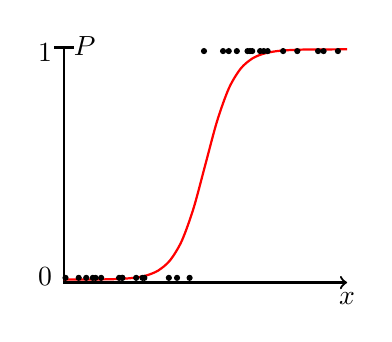
\begin{tikzpicture}[scale=0.15]
	\draw [thick, |->] (-12, 10) node [anchor=west] {\( P \)} -- (-12, -10) -- (12, -10) node [anchor=north] {\( x \)};
	\draw [red, thick, smooth] plot [domain=-12:12] (\x, {(1 / (1 + exp(-0.8*\x)))*19.5 - 9.75});
	\draw plot [only marks, mark=*, mark size=6, domain=-8:8, samples=15] ({12.5*rnd - 0.5}, 9.6);
	\draw plot [only marks, mark=*, mark size=6, domain=-8:8, samples=15] ({-12.5*rnd + 0.5}, -9.6);
	\draw (-15, -9.5) node [anchor=west] {0};
	\draw (-15, 9.5) node [anchor=west] {1};
\end{tikzpicture}

\end{multicols}

\columnbreak

\section*{Forma funcional incorrecta}

\textbf{Ramsey's RESET} (Regression Specification Error Test).

\begin{center}
	\( H_{0} \): el modelo está correctamente especificado.
\end{center}

\begin{enumerate}[leftmargin=*]
	\item Estimar el modelo original y obtener  \( \hat{y} \) y \( R^{2} \):
	\begin{center}
		\( \hat{y} = \hat{\beta}_{0} + \hat{\beta}_{1} x_{1} + \cdots + \hat{\beta}_{k} x_{k} \)
	\end{center}
	\item Estimar modelo con potencias de \( \hat{y} \) y obtener \( R_{\text{new}}^{2} \):
	\begin{center}
		\( \tilde{y} = \hat{y} + \tilde{\gamma}_{2} \hat{y}^{2} + \cdots + \tilde{\gamma}_{l} \hat{y}^{l} \)
	\end{center}
	\item Estadístico, bajo \( \gamma_{2} = \cdots = \gamma_{l} = 0 \) como \( H_{0} \):
	\begin{center}
		\( F = \frac{R_{\text{new}}^{2} - R^{2}}{1 - R_{\text{new}}^{2}} \cdot \frac{n - (k + 1) - l}{l} \sim F_{l, n - (k + 1) - l} \)
	\end{center}
\end{enumerate}

Si \( F > F_{l, n - (k + 1) - l} \), hay evidencia para rechazar \( H_{0} \).

\section*{Definiciones estadísticas}

Sean \( \xi, \eta \) variables aleatorias, \( a, b \in \mathbb{R} \) constantes, y \( P \) denota probabilidad.

\textbf{Media} \quad \( E(\xi) = \sum_{i = 1}^{n} \xi_{i} \cdot P[\xi = \xi_{i}] \)

Media muestral: \quad \( \E(\xi) = \dfrac{1}{n} \sum_{i = 1}^{n} \xi_{i} \)

Propiedades de la media:

\begin{itemize}[leftmargin=*]
	\item \( \E(a) = a \)
	\item \( \E(\xi + a) = \E(\xi) + a \)
	\item \( \E(a \cdot \xi) = a \cdot \E(\xi) \)
	\item \( \E(\xi \pm \eta) = \E(\xi) + \E(\eta) \)
	\item \( \E(\xi \cdot \eta) = \E(\xi) \cdot \E(\eta) \) \quad sólo si \( \xi \) y \( \eta \) son independientes.
	\item \( \E(\xi - \E(\xi)) = 0 \)
	\item \( \E(a \cdot \xi + b \cdot \eta) = a \cdot \E(\xi) + b \cdot \E(\eta) \)
\end{itemize}

\textbf{Varianza} \quad \( \Var(\xi) = \E \left[ (\xi - \E(\xi))^{2} \right] \)

Varianza muestral: \quad \( \Var(\xi) = \dfrac{\sum_{i = 1}^{n} (\xi_{i} - \E(\xi))^2}{n - 1} \)

Propiedades de la varianza:

\begin{itemize}[leftmargin=*]
	\item \( \Var(a) = 0 \)
	\item \( \Var(\xi + a) = \Var(\xi) \)
	\item \( \Var(a \cdot \xi) = a^{2} \cdot \Var(\xi) \)
	\item \( \Var(\xi \pm \eta) = \Var(\xi) + \Var(\eta) \pm 2 \cdot \Cov(\xi, \eta) \)
	\item \( \Var(a \cdot \xi \pm b \cdot \eta) = a^{2} \cdot \Var(\xi) + b^{2} \cdot \Var(\eta) \pm 2 a b \cdot \Cov(\xi, \eta) \)
\end{itemize}

\textbf{Covarianza} \quad \( \Cov(\xi, \eta) = \E \left[ (\xi - E(\xi)) \cdot (\eta - E(\eta)) \right] \)

Covarianza muestral: \quad \( \dfrac{\sum_{i = 1}^{n} (\xi_{i} - \E(\xi)) \cdot (\eta_{i} - \E(\eta))}{n - 1} \)

Propiedades de la covarianza:

\begin{itemize}[leftmargin=*]
	\item \( \Cov(\xi, a) = 0 \)
	\item \( \Cov(\xi + a, \eta + b) = \Cov(\xi, \eta) \)
	\item \( \Cov(a \cdot \xi, b \cdot \eta) = a b \cdot \Cov(\xi, \eta) \)
	\item \( \Cov(\xi, \xi) = \Var(\xi) \)
	\item \( \Cov(\xi, \eta) = \Cov(\eta, \xi) \)
\end{itemize}

\columnbreak

\section*{Contraste de hipótesis}

\begin{center}
	\begin{tabular}{ c | c | c }
		                        & \( H_{0} \) verdadera       & \( H_{0} \) falsa           \\ \hline
		Rechazar \( H_{0} \)    & Falso positivo              & Verdadero pos.              \\
		                        & Error Tipo I \( (\alpha) \) & \( (1 - \beta) \)           \\ \hline
		No rechazar \( H_{0} \) & Verdadero neg.              & Falso negativo              \\
		                        & \( (1 - \alpha) \)          & Error Tipo II \( (\beta) \)
	\end{tabular}
\end{center}

\columnbreak

Típico contraste de una cola:

\begin{center}
	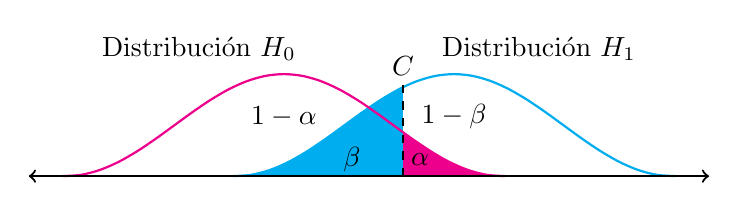
\begin{tikzpicture}[scale=0.108]
		\fill [magenta] (4, 0) -- plot [domain=4:16, smooth] (\x, {cos(\x*7 + 70)*6 + 6}); 
		\fill [cyan] (4, 0) -- plot [domain=-16:4, smooth] (\x, {cos(\x*7 - 70)*6 + 6}); 
		\draw [thick, cyan] plot [domain=-16:36, smooth] (\x, {cos(\x*7 - 70)*6 + 6}); 
		\draw [thick, magenta] plot [domain=-36:16, smooth] (\x, {cos(\x*7 + 70)*6 + 6}); 
		\draw [thick, <->] (-40, 0) -- (40, 0); 
		\draw [thick, dashed] (4, 0) -- (4, 11); 
		\node at (-20, 15) {Distribución \( H_{0} \)};
		\node at (20, 15) {Distribución \( H_{1} \)}; 
		\node at (-10, 7) {\( 1 - \alpha \)}; 
		\node at (10, 7) {\( 1 - \beta \)}; 
		\node at (6, 2) {\( \alpha \)}; 
		\node at (-2, 2) {\( \beta \)}; 
		\node at (4, 13) {\( C \)};
	\end{tikzpicture}
\end{center}

donde \( (1 - \alpha) \) es nivel de confianza, \( \alpha \) es nivel de significación, \( C \) es valor crítico, \( (1 - \beta) \) es potencia estadística.

\section*{Bootstraping}

\textbf{Problema} - Aprox. asint. a las distribuciones de los estadísticos de contraste no funcionan en muestras pequeñas.

\textbf{Solución} - Boostrap es muestreo con reemplazo. Los datos observados se tratan como una población y se extraen varias muestras para recalcular un estimador o estadístico varias veces (mejora la precisión).

\end{multicols}

\begin{multicols}{2}

\section*{VAR (Vector Autoregressive)}

Un modelo VAR captura \textbf{interacciones dinámicas} entre series temporales. El \( \text{VAR}(p) \):

\begin{center}
	\( y_{t} = A_{1} y_{t - 1} + \cdots + A_{p} y_{t - p} + B x_{t} + CD_{t} + u_{t} \)
\end{center}

donde:

\begin{itemize}[leftmargin=*]
	\item \( y_{t} = (y_{1t}, \ldots, y_{Kt})^{\top} \) es un vector de \( K \) series temporales observables endógenas.
	\item \( A_{i} \)'s son \( K \times K \) matrices de coeficientes.
	\item \( x_{t} = (x_{1t}, \ldots, x_{Mt})^{\top} \) es un vector de \( M \) series temporales observables exógenas.
	\item \( B \) es una matriz de coeficientes \( K \times M \).
	\item \( D_{t} \) es un vector que contiene los términos deterministas: una constante, tendencia lineal, variables estacionales binarias, y/o cualquier otra variable ficticia especificada.
	\item \( C \) es una matriz de coeficientes de dimensión apropiada.
	\item \( u_{t} = (u_{1t}, \ldots, u_{Kt})^{\top} \) es un vector de \( K \) series de ruido blanco.
\end{itemize}

\textbf{Condición de estabilidad}:

\begin{center}
	\( \det(I_{K} - A_{1} z - \cdots - A_{p} z^{p}) \neq 0 \quad \text{para}\quad \lvert z \rvert \leq 1 \)
\end{center}

\quad esto es, \textbf{no hay raíces} en y sobre el círculo unitario complejo.

Por ejemplo, un modelo VAR con dos variables endógenas \( (K = 2) \), dos retardos \( (p = 2) \), una variable exógena contemporánea \( (M = 1) \), constante \( (\const) \) y tendencia \( (\trend) \):

\begin{center}
	\scalebox{0.80}{
		\(
		\begin{bmatrix}
			y_{1t} \\
			y_{2t}
		\end{bmatrix}
		=
		\begin{bmatrix}
			a_{11, 1} & a_{12, 1} \\
			a_{21, 1} & a_{22, 1}
		\end{bmatrix}
		\cdot
		\begin{bmatrix}
			y_{1, t - 1} \\
			y_{2, t - 1}
		\end{bmatrix}
		+
		\begin{bmatrix}
			a_{11, 2} & a_{12, 2} \\
			a_{21, 2} & a_{22, 2}
		\end{bmatrix}
		\cdot
		\begin{bmatrix}
			y_{1, t - 2} \\
			y_{2, t - 2}
		\end{bmatrix}
		+
		\begin{bmatrix}
			b_{11} \\
			b_{21}
		\end{bmatrix}
		\cdot
		\begin{bmatrix}
			x_{t}
		\end{bmatrix}
		+
		\begin{bmatrix}
			c_{11} & c_{12} \\
			c_{21} & c_{22}
		\end{bmatrix}
		\cdot
		\begin{bmatrix}
			\const \\
			\trend
		\end{bmatrix}
		+
		\begin{bmatrix}
			u_{1t} \\
			u_{2t}
		\end{bmatrix}
		\)
	}
\end{center}

Visualizando las ecuaciones por separado:

\begin{center}
	\( y_{1t} = a_{11, 1} y_{1, t - 1} + a_{12, 1} y_{2, t - 1} + a_{11, 2} y_{1, t - 2} + a_{12, 2} y_{2, t - 2} + b_{11} x_{t} + c_{11} + c_{12} \trend + u_{1t} \)

	\( y_{2t} = a_{21, 1} y_{2, t - 1} + a_{22, 1} y_{1, t - 1} + a_{21, 2} y_{2, t - 2} + a_{22, 2} y_{1, t - 2} + b_{21} x_{t} + c_{21} + c_{22} \trend + u_{2t} \)
\end{center}

Si hay una raíz unitaria, el determinante es cero para \( z = 1 \); entonces una o todas las variables son integrados, y el modelo VAR ya no es apropiado (es inestable).

\subsection*{SVAR (Structural VAR)}

En un modelo VAR, las interpretaciones de causalidad no son explícitas, y los resultados pueden variar según el orden de las variables. Un SVAR extiende el VAR al imponer restricciones sobre las matrices \( \mathsf{A} \) y/o \( \mathsf{B} \). Esto permite una interpretación causal y un análisis de shocks sin necesidad de depender de un orden arbitrario.

Por ejemplo, un modelo \( \text{SVAR}(p) \) básico:

\begin{center}
	\( \mathsf{A} y_t = \mathsf{A} [A_1, \ldots, A_p] y_{t - 1} + \mathsf{B} \varepsilon_t \)
\end{center}

donde:

\begin{itemize}[leftmargin=*]
	\item \( u_t = \mathsf{A}^{-1} \mathsf{B} \varepsilon_t \)
	\item \( \mathsf{A} \), \( \mathsf{B} \) son \( (K \times K) \) matrices.
\end{itemize}

\columnbreak

\section*{VECM (Vector Error Correction Model)}

Si existen \textbf{relaciones cointegradoras} en un sistema de variables, la forma VAR no es la más conveniente. Es mejor usar un VECM, esto es, el VAR en niveles, sustrayendo \( y_{t - 1} \) de ambos lados. El \( \text{VECM}(p - 1) \):

\begin{center}
	\( \Delta y_{t} = \Pi y_{t - 1} + \sum_{i = 1}^{p - 1} \Gamma_{i} \Delta y_{t - i} + B x_{t} + CD_{t} + u_{t} \)
\end{center}

donde:

\begin{itemize}[leftmargin=*]
	\item \( \Delta y_{t} = (\Delta y_{1t}, \ldots, \Delta y_{Kt})^{\top} \) es un vector de \( K \) series temporales observables endógenas.
	\item \( \Pi y_{t - 1} \) es la parte \textbf{largo plazo}.
	\begin{itemize}[leftmargin=*, label={\( \diamond \)}]
		\item \( \Pi = - (I_{K} - A_{1} - \cdots - A_{p}) \) para \( i = 1, \ldots, p - 1 \)
		\item \( \Pi = \alpha \beta^{\top} \)
		\item \( \alpha \) es la \textbf{matriz de carga} \( (K \times r) \). Representa la velocidad de ajuste.
		\item \( \beta \) es la \textbf{matriz de cointegración} \( (K \times r) \).
		\item \( \beta^{\top} y_{t - 1} \) es la \textbf{ecuación de cointegración}. Representa el equilibrio a largo plazo.
		\item \( \rk(\Pi) = \rk(\alpha) = \rk(\beta) = r \) es el \textbf{rango cointegrador}.
	\end{itemize}
	\item \( \Gamma_{i} = - (A_{i + 1} + \cdots + A_{p}) \) para \( i = 1, \ldots, p - 1 \) son los parámetros a \textbf{corto plazo}.
	\item \( x_{t} \), \( B \), \( C \), \( D_{t} \) y \( u_{t} \) son como en VAR.
\end{itemize}

Por ejemplo, un VECM con tres variables endógenas \( (K = 3) \), dos retardos \( (p = 2) \) y dos relaciones cointegradoras \( (r = 2) \):

\begin{center}
	\( \Delta y_{t} = \Pi y_{t - 1} + \Gamma_{1} \Delta y_{t - 1} + u_{t} \)
\end{center}

\quad donde:

\begin{center}
	\scalebox{0.95}{
		\(
		\Pi y_{t - 1} = \alpha \beta^{\top} y_{t - 1} =
		\begin{bmatrix}
			\alpha_{11} & \alpha_{12} \\
			\alpha_{21} & \alpha_{22} \\
			\alpha_{31} & \alpha_{32}
		\end{bmatrix}
		\begin{bmatrix}
			\beta_{11} & \beta_{21} & \beta_{31} \\
			\beta_{12} & \beta_{22} & \beta_{32}
		\end{bmatrix}
		\begin{bmatrix}
			y_{1, t - 1} \\
			y_{2, t - 1} \\
			y_{3, t - 1}
		\end{bmatrix}
		=
		\begin{bmatrix}
			\alpha_{11} ec_{1, t - 1} + \alpha_{12} ec_{2, t - 1} \\
			\alpha_{21} ec_{1, t - 1} + \alpha_{22} ec_{2, t - 1} \\
			\alpha_{31} ec_{1, t - 1} + \alpha_{32} ec_{2, t - 1}
		\end{bmatrix}
		\)
	}
\end{center}

\vspace*{0.2cm}

\begin{center}
	\( ec_{1, t - 1} = \beta_{11} y_{1, t - 1} + \beta_{21} y_{2, t - 1} + \beta_{31} y_{3, t - 1} \)

	\( ec_{2, t - 1} = \beta_{12} y_{1, t - 1} + \beta_{22} y_{2, t - 1} + \beta_{32} y_{3, t - 1} \)
\end{center}

\quad y

\begin{center}
	\scalebox{0.95}{
		\(
		\Gamma_{1} \Delta y_{t - 1} = 
		\begin{bmatrix}
			\gamma_{11} & \gamma_{12} & \gamma_{13} \\
			\gamma_{21} & \gamma_{22} & \gamma_{23} \\
			\gamma_{31} & \gamma_{32} & \gamma_{33}
		\end{bmatrix}
		\begin{bmatrix}
			\Delta y_{1, t - 1} \\
			\Delta y_{2, t - 1} \\
			\Delta y_{3, t - 1}
		\end{bmatrix}
		\quad
		u_t =
		\begin{bmatrix}
			u_{1} \\
			u_{2} \\
			u_{3}
		\end{bmatrix}
		\)
	}
\end{center}

Visualizando las ecuaciones por separado:

\begin{center}
	\( \Delta y_{1t} = \alpha_{11} ec_{1, t - 1} + \alpha_{12} ec_{2, t - 1}  + \gamma_{11} \Delta y_{1, t - 1} + \gamma_{12} \Delta y_{2, t - 1} + \gamma_{13} \Delta y_{3, t - 1} + u_{1t} \)

	\( \Delta y_{2t} = \alpha_{21} ec_{1, t - 1} + \alpha_{22} ec_{2, t - 1}  + \gamma_{21} \Delta y_{1, t - 1} + \gamma_{22} \Delta y_{2, t - 1} + \gamma_{23} \Delta y_{3, t - 1} + u_{2t} \)

	\( \Delta y_{3t} = \alpha_{31} ec_{1, t - 1} + \alpha_{32} ec_{2, t - 1}  + \gamma_{31} \Delta y_{1, t - 1} + \gamma_{32} \Delta y_{2, t - 1} + \gamma_{33} \Delta y_{3, t - 1} + u_{3t} \)
\end{center}

\end{multicols}

\end{document}